\documentclass[10pt]{beamer}\usepackage[]{graphicx}\usepackage[]{color}
% maxwidth is the original width if it is less than linewidth
% otherwise use linewidth (to make sure the graphics do not exceed the margin)
\makeatletter
\def\maxwidth{ %
  \ifdim\Gin@nat@width>\linewidth
    \linewidth
  \else
    \Gin@nat@width
  \fi
}
\makeatother

\definecolor{fgcolor}{rgb}{0.345, 0.345, 0.345}
\makeatletter
\@ifundefined{AddToHook}{}{\AddToHook{package/xcolor/after}{\definecolor{fgcolor}{rgb}{0.345, 0.345, 0.345}}}
\makeatother
\newcommand{\hlnum}[1]{\textcolor[rgb]{0.686,0.059,0.569}{#1}}%
\newcommand{\hlstr}[1]{\textcolor[rgb]{0.192,0.494,0.8}{#1}}%
\newcommand{\hlcom}[1]{\textcolor[rgb]{0.678,0.584,0.686}{\textit{#1}}}%
\newcommand{\hlopt}[1]{\textcolor[rgb]{0,0,0}{#1}}%
\newcommand{\hlstd}[1]{\textcolor[rgb]{0.345,0.345,0.345}{#1}}%
\newcommand{\hlkwa}[1]{\textcolor[rgb]{0.161,0.373,0.58}{\textbf{#1}}}%
\newcommand{\hlkwb}[1]{\textcolor[rgb]{0.69,0.353,0.396}{#1}}%
\newcommand{\hlkwc}[1]{\textcolor[rgb]{0.333,0.667,0.333}{#1}}%
\newcommand{\hlkwd}[1]{\textcolor[rgb]{0.737,0.353,0.396}{\textbf{#1}}}%
\let\hlipl\hlkwb

\usepackage{framed}
\makeatletter
\newenvironment{kframe}{%
 \def\at@end@of@kframe{}%
 \ifinner\ifhmode%
  \def\at@end@of@kframe{\end{minipage}}%
  \begin{minipage}{\columnwidth}%
 \fi\fi%
 \def\FrameCommand##1{\hskip\@totalleftmargin \hskip-\fboxsep
 \colorbox{shadecolor}{##1}\hskip-\fboxsep
     % There is no \\@totalrightmargin, so:
     \hskip-\linewidth \hskip-\@totalleftmargin \hskip\columnwidth}%
 \MakeFramed {\advance\hsize-\width
   \@totalleftmargin\z@ \linewidth\hsize
   \@setminipage}}%
 {\par\unskip\endMakeFramed%
 \at@end@of@kframe}
\makeatother

\definecolor{shadecolor}{rgb}{.97, .97, .97}
\definecolor{messagecolor}{rgb}{0, 0, 0}
\definecolor{warningcolor}{rgb}{1, 0, 1}
\definecolor{errorcolor}{rgb}{1, 0, 0}
\makeatletter
\@ifundefined{AddToHook}{}{\AddToHook{package/xcolor/after}{
\definecolor{shadecolor}{rgb}{.97, .97, .97}
\definecolor{messagecolor}{rgb}{0, 0, 0}
\definecolor{warningcolor}{rgb}{1, 0, 1}
\definecolor{errorcolor}{rgb}{1, 0, 0}
}}
\makeatother
\newenvironment{knitrout}{}{} % an empty environment to be redefined in TeX

\usepackage{alltt}

\beamertemplatenavigationsymbolsempty

\usepackage{booktabs}
\usepackage{colortbl}

\usepackage{tikz}
\usetikzlibrary{positioning,shapes.misc,calc,backgrounds,scopes} 
\tikzset{boxed/.style={
  thick,
  draw=black,
  top color=white,
  text height=1.5ex,
  text depth=.25ex
}}


\newcommand\lo{\ensuremath{\boldsymbol{-}}}
\newcommand\hi{\ensuremath{\boldsymbol{+}}}

\title{Process Improvement: Steepest Ascent}
\author{BIOE 498/598 PJ}
\date{Spring 2022}
\IfFileExists{upquote.sty}{\usepackage{upquote}}{}
\begin{document}
\frame{\titlepage}

\begin{frame}{Process Improvement}

Design of Experiments is focused on \textbf{process characterization}.
\begin{itemize}
  \item Which factors affect the response?
  \item How large are the effects?
\end{itemize}

\bigskip
\pause
\textbf{Process improvement} asks ``what factor settings yield the optimal response?''

\begin{center}
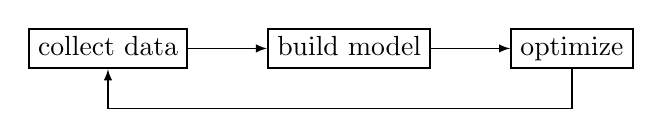
\begin{tikzpicture}[>=latex]
  \node (collect) [boxed] {collect data};
  \node (build) [boxed,right=of collect] {build model};
  \node (optimize) [boxed,right=of build] {optimize};
  \draw [->] (collect) -- (build);
  \draw [->] (build) -- (optimize);
  \draw [->] (optimize.south) -- ++(0,-0.5) -| (collect.south);
\end{tikzpicture}
\end{center}

\end{frame}

\begin{frame}{Surrogate Optimization}

\begin{center}
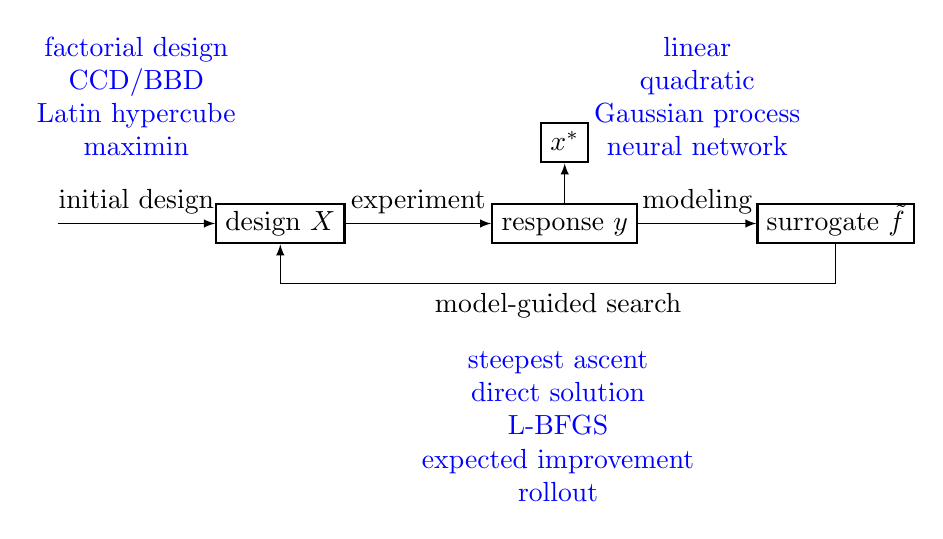
\begin{tikzpicture}[>=latex]
  \node (start) {};
  \node (data) [boxed, right=2cm of start] {design $X$};
  \node (response) [boxed,right=1.85cm of data] {response $y$};
  \node (optimal) [boxed,above=0.5cm of response] {$x^*$};
  \draw [->] (start) -- (data) node [midway,above] (initial) {initial design};
  \draw [->] (data) -- (response) node [midway,above] {experiment};
  \draw [->] (response) -- (optimal);
  
  \onslide<2->{
    \node (surrogate) [boxed,right=1.5cm of response] {surrogate $\tilde{f}$};
    \draw [->] (response) -- (surrogate) node [midway,above] (modeling) {modeling};
  }
  \onslide<3->{
    \draw [->] (surrogate.south) -- ++(0,-0.5) -| (data.south) node [near start,below] (search) {model-guided search};
  }
  
  \onslide<4->{
    \node [blue,align=center,above=0.5em of initial] {factorial design\\CCD/BBD\\Latin hypercube\\maximin};
    \node [blue,align=center,above=0.5em of modeling] {linear\\quadratic\\Gaussian process\\neural network};
    \node [blue,align=center,below=0.5em of search] {steepest ascent\\direct solution\\L-BFGS\\expected improvement\\rollout};
  }
\end{tikzpicture}
\end{center}

\end{frame}

\begin{frame}{Process improvement by steepest ascent}

\begin{itemize}
  \item Rarely are the initial factor ranges optimal. In practice we can be far away.
  \item<2-> The \textbf{method of steepest ascent} moves us quickly toward regions of better response.
  \item<3-> The emphasis is on moving quickly using few runs and first order models.
\end{itemize}

\end{frame}

\begin{frame}{The Design Space}

Runs in a factorial design sample the corners of a unit cube.
\bigskip

\begin{center}
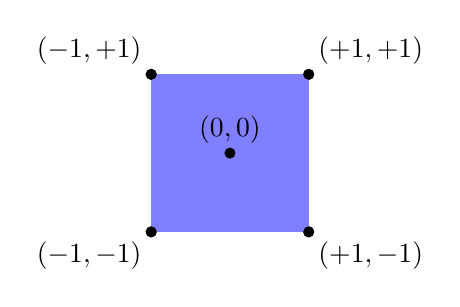
\begin{tikzpicture}

\fill [black] (1,1) circle (2pt)
              (1,-1) circle (2pt)
              (-1,1) circle (2pt)
              (-1,-1) circle (2pt);
\draw (1,1) node [above right] {$(+1,+1)$}
      (1,-1) node [below right] {$(+1,-1)$}
      (-1,1) node [above left] {$(-1,+1)$}
      (-1,-1) node [below left] {$(-1,-1)$};

\draw (-1,-1) rectangle (1,1);

\onslide<2->{
  \fill [fill=blue!50] (-1,-1) rectangle (1,1);
  \fill [black] (1,1) circle (2pt)
              (1,-1) circle (2pt)
              (-1,1) circle (2pt)
              (-1,-1) circle (2pt);
}

\onslide<3->{
  \fill [black] (0,0) circle (2pt);
  \node [above] (0,0) {$(0,0)$};
}

\end{tikzpicture}
\end{center}

\bigskip
\onslide<2->{The region inside the factorial points is called the \textbf{design space}.}

\onslide<3->{The origin $(0,0)$ in \emph{coded units} is called the \textbf{center point}.}

\end{frame}

\begin{frame}{Model Distance}

\begin{itemize}
  \item<1-> A linear model averages over runs at all corners of the design space.
  \item<2-> The model's predictions are best at the center point.
  \item<3-> As we move away from the center point, we switch from \emph{interpolating} to \emph{extrapolating}.
  \item<4-> The \textbf{design radius} measures how far we are from the center point.
\end{itemize}

\begin{columns}

\begin{column}{0.5\textwidth}<4->
  \begin{center}
    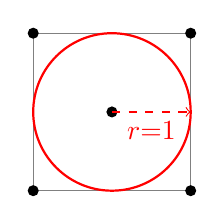
\begin{tikzpicture}
        \draw [help lines] (1,1) -- (-1,1) -- (-1,-1) -- (1,-1) -- cycle;
        \fill [black] 
                  (0,0) circle (2pt)
                  (1,1) circle (2pt)
                  (1,-1) circle (2pt)
                  (-1,1) circle (2pt)
                  (-1,-1) circle (2pt);
        \draw [thick,red] (0,0) circle (1);
        \draw [red,dashed,->] (0,0) -- (1,0) node [midway,below] {$r$=1};
    \end{tikzpicture}
    
    $r=1$ touches the \emph{faces} of the design space
  \end{center}
\end{column}

\begin{column}{0.5\textwidth}<5->
  \begin{center}
    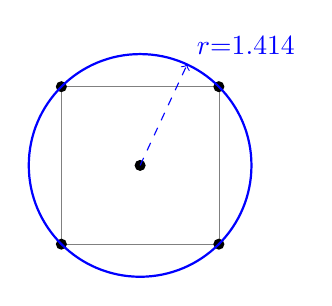
\begin{tikzpicture}
        \draw [help lines] (1,1) -- (-1,1) -- (-1,-1) -- (1,-1) -- cycle;
        \fill [black] 
                  (0,0) circle (2pt)
                  (1,1) circle (2pt)
                  (1,-1) circle (2pt)
                  (-1,1) circle (2pt)
                  (-1,-1) circle (2pt);
        \draw [thick,blue] (0,0) circle (1.414);
        \draw [blue,dashed,->,rotate=65] (0,0) -- (1.414,0) node [above right] {$r$=1.414};
    \end{tikzpicture}
    
    $r=\sqrt{2}\approx 1.414$ touches the factorial points
  \end{center}
\end{column}

\end{columns}

\end{frame}

\begin{frame}[fragile]{First-order response surfaces}

Consider the first-order linear model (without interactions)
\[ y = 20 + 3.6x_1 - 1.8x_2 \]

\begin{columns}

\begin{column}{0.5\textwidth}<2->
\begin{knitrout}
\definecolor{shadecolor}{rgb}{0.969, 0.969, 0.969}\color{fgcolor}

{\centering 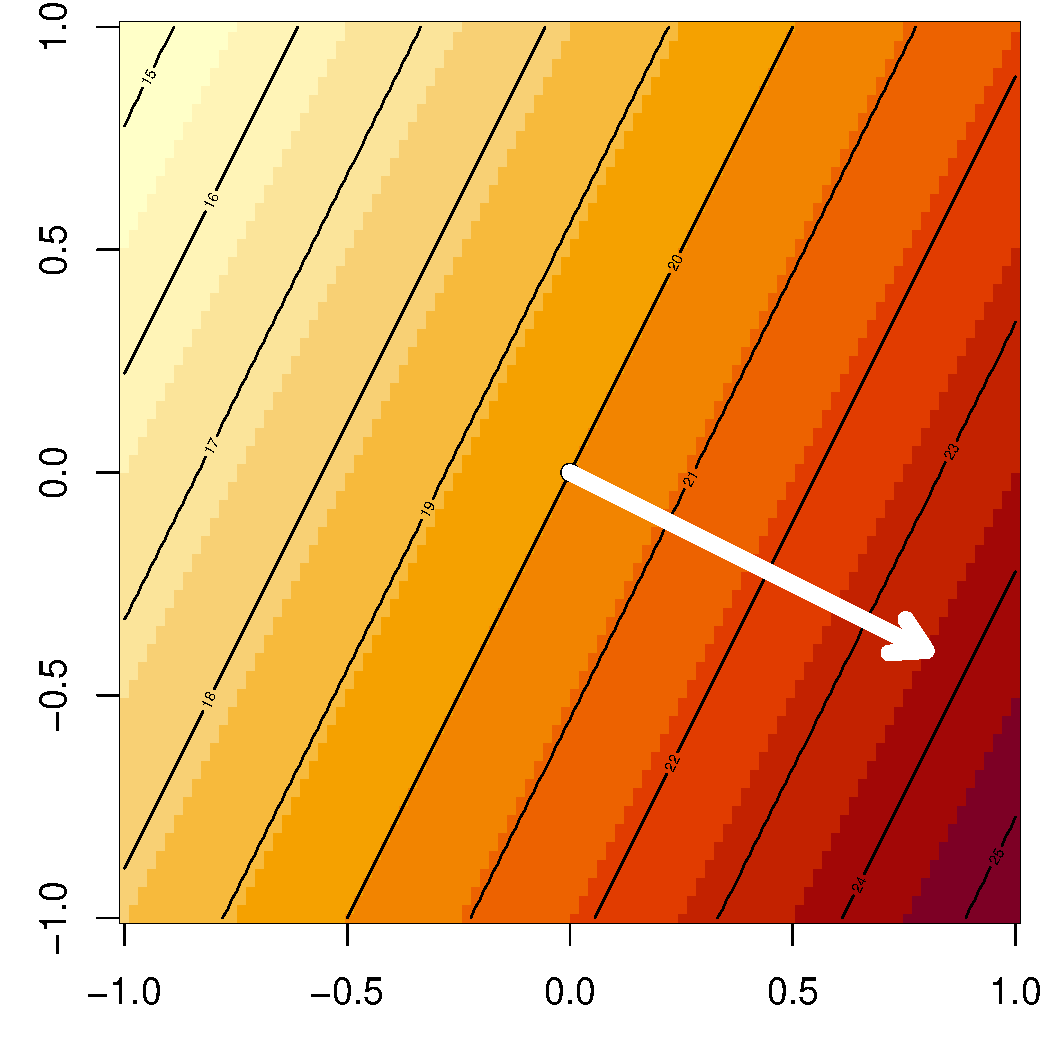
\includegraphics[width=\textwidth]{figure/unnamed-chunk-1-1} 

}


\end{knitrout}

\end{column}

\begin{column}{0.5\textwidth}<3->
We want to move ``uphill'' to improve the response using the \textbf{method of steepest ascent}.

\bigskip
If our goal was to minimize the response, we use \emph{steepest descent} by
\begin{enumerate}
  \item Moving opposite of the uphill direction, or
  \item Multiplying the response by $-1$.
\end{enumerate}
\end{column}

\end{columns}

\end{frame}

\begin{frame}{Finding the ascent direction for first-order models}

Let's compute the partial derivatives along each factor's dimension.

\begin{align*}
  \frac{\partial y}{\partial x_1} &= \frac{\partial}{\partial x_1}\left( 20 + 3.6x_1 - 1.8x_2 \right) = 3.6 \\
  \frac{\partial y}{\partial x_2} &= \frac{\partial}{\partial x_2}\left( 20 + 3.6x_1 - 1.8x_2 \right) = -1.8
\end{align*}

\pause
\bigskip
Two things to note:
\begin{enumerate}
  \item The rate of ascent along each direction is simply the effect size $\beta_i$.
  \item The rate of change is different for the two dimensions. For every step of unit length along $x_1$ we must move $-1.8/3.6=-1/2$ units along $x_2$.
\end{enumerate}

\end{frame}

\begin{frame}{Standardized step sizes for steepest ascent}

Consider the general first-order model
\[ y = \beta_0 + \beta_1x_1 + \beta_2x_2 + \cdots + \beta_nx_n \]

\begin{enumerate}
  \item Find the effect size with the largest \textbf{magnitude}. We'll call this $\beta_j$ and the associated factor $x_j$.
  \item Choose a step size (in coded units) along this dimension, called $\Delta x_j$.
  \item For all other dimensions $i\ne j$, the step size is
    \[ \Delta x_i = \frac{\beta_i}{\beta_j}\Delta x_j \]
\end{enumerate}

\pause
\textbf{Example:} $y = 20 + 3.6x_1 - 1.8x_2$.
\begin{enumerate}
  \item<3-> $|3.6| > |-1.8|$, so we standardize using $x_1$ ($j\equiv1$).
  \item<4-> Let $\Delta x_1=1$.
  \item<5-> $\Delta x_2 = \frac{\beta_2}{\beta_1}\Delta x_1 = \frac{-1.8}{3.6}(1) = -0.5$
\end{enumerate}

\end{frame}

\begin{frame}{Why standardize step sizes?}

\begin{columns}
\begin{column}{0.5\textwidth}
\begin{center}
Uniform steps give uniform differences in design radii.

\bigskip
  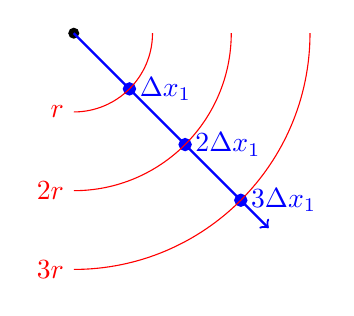
\begin{tikzpicture}
    \fill [black] (0,0) circle (2pt);
    \draw [thick,blue,rotate=-45,->] 
      (0,0) -- (3.5,0);
    \filldraw [thick,blue,rotate=-45]
      (1,0) circle (2pt) node [right] {$\Delta x_1$} 
      (2,0) circle (2pt) node [right] {$2\Delta x_1$}
      (3,0) circle (2pt) node [right] {$3\Delta x_1$};
    \onslide<2->{
      \draw [red] (1,0) arc (0:-90:1) node [left] {$r$};
      \draw [red] (2,0) arc (0:-90:2) node [left] {$2r$};
      \draw [red] (3,0) arc (0:-90:3) node [left] {$3r$};
    }
  \end{tikzpicture}
\end{center}

\end{column}

\begin{column}{0.5\textwidth}<3->
\begin{center}
  A standardized step of 1 always defines a point on the design space boundary.

  \bigskip
  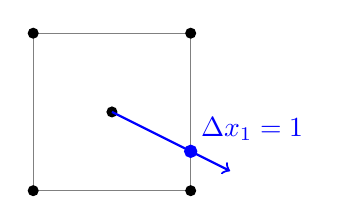
\begin{tikzpicture}
      \draw [help lines] (1,1) -- (-1,1) -- (-1,-1) -- (1,-1) -- cycle;
      \fill [black] 
                (0,0) circle (2pt)
                (1,1) circle (2pt)
                (1,-1) circle (2pt)
                (-1,1) circle (2pt)
                (-1,-1) circle (2pt);
      \draw [thick,blue,->] (0,0) -- (1.5,-0.75);
      \filldraw [thick,blue] (1,-0.5) circle (2pt) node [above right] {$\Delta x_1 = 1$};
  \end{tikzpicture}
\end{center}

\end{column}
\end{columns}
\end{frame}

\begin{frame}{How far do we go?}

\begin{columns}
\begin{column}{0.5\textwidth}
  \begin{itemize}
    \item A first order model predicts the response will increase \emph{forever}.
    \item We perform additional runs at every step along the ascent path.
    \item<2-> The first run is close to the center to confirm the system behaves as expected.
    \item<3-> Eventually the actual response will stop increasing.
    \item<4-> When the response drifts, we use the best response location as the center for a new set of experiments.
  \end{itemize}
\end{column}
\begin{column}{0.5\textwidth}
  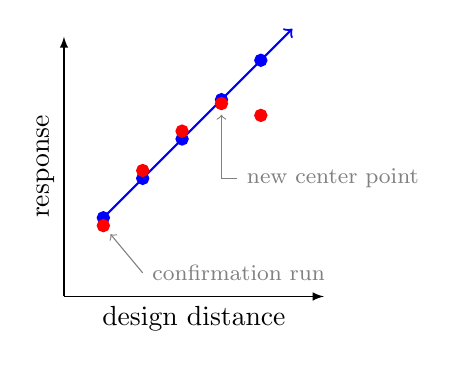
\begin{tikzpicture}
    \draw [>=latex,->] (0,0) -- (3.3,0) node [midway,below] {design distance};
    \draw [>=latex,->] (0,0) -- (0,3.3) node [midway,left,anchor=south,rotate=90] {response};
    \filldraw [thick,blue] 
         (0.5,1.0) circle (2pt) 
      -- (1.0,1.5) circle (2pt)
      -- (1.5,2.0) circle (2pt)
      -- (2.0,2.5) circle (2pt)
      -- (2.5,3.0) circle (2pt);
    \filldraw [thick,blue,->] (2.5,3.0) -- (2.9,3.4);
    \onslide<2->{
      \filldraw [thick,red]
           (0.5,0.9) circle (2pt);
      \draw [gray,->,shorten >=4pt] (1,0.3) -- (0.5,0.9);
      \node [gray,right] at (1,0.3) {\footnotesize confirmation run};
    }
    \onslide<3->{
      \filldraw [thick,red]
           (1.0,1.6) circle (2pt)
           (1.5,2.1) circle (2pt)
           (2.0,2.45) circle (2pt)
           (2.5,2.3) circle (2pt);
    }
    \onslide<4->{
      \draw [gray,->,shorten >=4pt] (2.2,1.5) -| (2.0,2.45);
      \node [gray,right] at (2.2,1.5) {\footnotesize new center point};
    }
  \end{tikzpicture}
\end{column}
\end{columns}

\end{frame}

\begin{frame}{What about interactions?}

Models with interactions have \textbf{curved} paths of steepest ascent since the gradient changes with $\boldsymbol{x}$.
\[ y = \beta_0 + \beta_1x_1 + \beta_2x_2 + \beta_{12}x_1x_2 \]

\[ \nabla y = \begin{pmatrix} \frac{\partial y}{\partial x_1} \\ \frac{\partial y}{\partial x_2} \end{pmatrix}
 = \begin{pmatrix} \beta_1 + \beta_{12}x_2 \\ \beta_2 + \beta_{12}x_1 \end{pmatrix} \]
 
 \pause
 We can follow this path by integrating: $\boldsymbol{x}_{k+1} = \boldsymbol{x}_k + (\nabla y)\Delta x$.

\pause
\bigskip
\textbf{However}, in practice we usually ignore the interactions.
\begin{itemize}
  \item The model will often break down before the curvature becomes significant.
  \item We rarely have enough runs in the initial design to identify interactions.
\end{itemize}

\end{frame}

\begin{frame}{When is a first order model not good enough?}

\begin{itemize}
\item The FF designs used for process improvement are usually augmented by \textbf{center points} --- repeated runs at the design center $(0,0)$. 
\item Center points serve two purposes:
\begin{enumerate}
  \item Estimate the \emph{pure error} via the standard deviation of the repeated runs.
  \item Test for \emph{lack of fit} to detect curvature.
\end{enumerate}
\end{itemize}

\begin{center}
  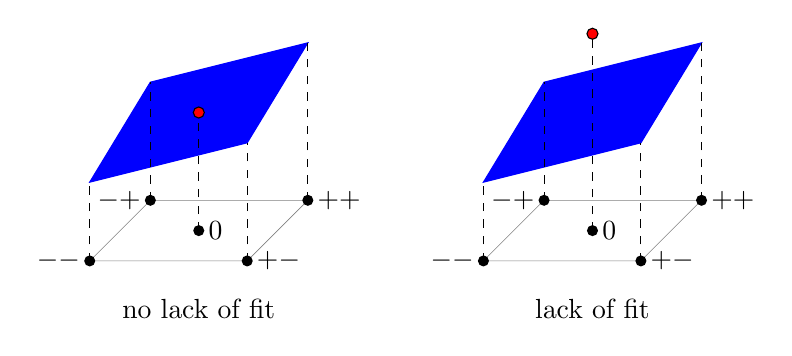
\begin{tikzpicture}
  \onslide<2->{
    \begin{scope}
      \coordinate (pm) at (1,0,1);
      \coordinate (pp) at (1,0,-1);
      \coordinate (mm) at (-1,0,1);
      \coordinate (mp) at (-1,0,-1);
      \coordinate (c) at (0,0,0);
      
      \coordinate (ypm) at ($(pm) +(0,1.5,0)$);
      \coordinate (ypp) at ($(pp) +(0,2,0)$);
      \coordinate (ymm) at ($(mm) +(0,1,0)$);
      \coordinate (ymp) at ($(mp) +(0,1.5,0)$);
    
      \draw [help lines] 
        (pp) -- (mp) -- (mm) -- (pm) -- cycle;
      
      \fill [black] 
        (pp) circle (2pt) node [right] {$++$}
        (pm) circle (2pt) node [right] {$+-$}
        (mp) circle (2pt) node [left] {$-+$}
        (mm) circle (2pt) node [left] {$--$}
        (c) circle (2pt) node [right] {$0$};
      
      \filldraw [blue] (ypp) -- (ymp) -- (ymm) -- (ypm) -- cycle;
      \draw [dashed] 
        (pp) -- (ypp)
        (pm) -- (ypm)
        (mp) -- (ymp)
        (mm) -- (ymm);
      
      \onslide<3->{
        \draw [dashed]
          (c) -- +(0,1.5,0);
        \filldraw [fill=red] ($(c) +(0,1.5,0)$) circle (2pt);
        \node at ($(c) + (0,-1,0)$) {no lack of fit};
      }
    \end{scope}
  }
  
  \onslide<4->{
    \begin{scope}[shift={(5,0)}]
      \coordinate (pm) at (1,0,1);
      \coordinate (pp) at (1,0,-1);
      \coordinate (mm) at (-1,0,1);
      \coordinate (mp) at (-1,0,-1);
      \coordinate (c) at (0,0,0);
      
      \coordinate (ypm) at ($(pm) +(0,1.5,0)$);
      \coordinate (ypp) at ($(pp) +(0,2,0)$);
      \coordinate (ymm) at ($(mm) +(0,1,0)$);
      \coordinate (ymp) at ($(mp) +(0,1.5,0)$);
      \draw [help lines] 
        (pp) -- (mp) -- (mm) -- (pm) -- cycle;
      
      \fill [black] 
        (pp) circle (2pt) node [right] {$++$}
        (pm) circle (2pt) node [right] {$+-$}
        (mp) circle (2pt) node [left] {$-+$}
        (mm) circle (2pt) node [left] {$--$}
        (c) circle (2pt) node [right] {$0$};
      
      \filldraw [blue] (ypp) -- (ymp) -- (ymm) -- (ypm) -- cycle;
      \draw [dashed] 
        (pp) -- (ypp)
        (pm) -- (ypm)
        (mp) -- (ymp)
        (mm) -- (ymm);
      
      \node at ($(c) + (0,-1,0)$) {lack of fit};
      
      \draw [dashed]
        (c) -- +(0,2.5,0);
      \filldraw [fill=red] ($(c) +(0,2.5,0)$) circle (2pt);
    \end{scope}
  }
  \end{tikzpicture}
\end{center}

\end{frame}

\begin{frame}{Testing for lack of fit due to curvature}

We want to compare the degree of curvature to the uncertainty (pure error) in our center points. We compare using a sum-of-squares approach.

\begin{enumerate}
  \item<2-> $\bar{y}_\text{center} = $ mean response of the $n_\text{center}$ center points\\ 
      $\bar{y}_\text{fact} = $ mean response of the $n_\text{fact}$ factorial points
  \item<3-> \[ SS_\text{curve} = \frac{n_\text{fact}n_\text{center}(\bar{y}_\text{fact} - \bar{y}_\text{center})^2}{n_\text{fact} + n_\text{center}},\quad \text{DF}(SS_\text{curve}) = 1 \]
  \item<4-> \[ SS_\text{error} = \sum_{\substack{\text{center} \\ \text{points}}} (y_i - \bar{y}_\text{center})^2,\quad \text{DF}(SS_\text{error}) = n_\text{center} - 1 \]
  \item<5-> \[ F_\text{curve} = \frac{SS_\text{curve}/\text{DF}(SS_\text{curve})}{SS_\text{error}/\text{DF}(SS_\text{error})} \]
\end{enumerate}

\end{frame}
{\small
\begin{frame}{Example: Testing for curvature (Myers 2009)}
\begin{columns}
\begin{column}{0.7\textwidth}
\begin{enumerate}
  \item<2-> $\bar{y}_\text{fact} = (39.3+40.0+40.9+41.5)/4 = 40.425$ \\
    $\bar{y}_\text{center} = (40.3+40.5+40.7+40.2+40.6)/5 = 40.46$
  \item<3-> \[ SS_\text{curve} = \frac{4\times 5\times(40.425 - 40.46)^2}{4+5} = 0.0026 \]
  \item<4-> \begin{align*}
    SS_\text{error} &= (40.3-40.46)^2 + \cdots + (40.6-40.46)^2 \\
                &= 0.172
    \end{align*}
  \item<5-> \[ F_\text{curve} = \frac{0.0026/1}{0.172/(5-1)} = 0.0605 \]
\end{enumerate}
\end{column}
\begin{column}{0.3\textwidth}

\begin{tabular}{ccc}
\toprule
temp & time & yield \\
\midrule
\lo & \lo & 39.3 \\
\lo & \hi & 40.0 \\
\hi & \lo & 40.9 \\
\hi & \hi & 41.5 \\
\midrule
0 & 0 & 40.3 \\
0 & 0 & 40.5 \\
0 & 0 & 40.7 \\
0 & 0 & 40.2 \\
0 & 0 & 40.6 \\
\bottomrule
\end{tabular}

\end{column}
\end{columns}

\bigskip
\onslide<6->{
  \texttt{pf(0.0605, 1, 4, lower.tail=FALSE)} $\rightarrow p < 0.818$.
}

\end{frame}
} %\small

\begin{frame}{The steepest ascent method}

\begin{enumerate}
  \item<1-> Run a FF design augmented with replicated center points.
  \item<2-> Fit a first order model and check for lack of fit.
    \begin{itemize}
      \item If significant lack of fit, switch to Response Surface Methodology.
    \end{itemize}
  \item<3-> Perform runs along the steepest ascent path until the response diminishes.
  \item<4-> Go to (1) and repeat using the location of maximum response as the new center point.
\end{enumerate}

\end{frame}

\end{document}
